\documentclass[12pt]{article}
\usepackage{graphicx} % Required for inserting images
\usepackage{amsthm}
\usepackage{amsmath}
\usepackage{amssymb}
\usepackage{hyperref}

\title{Stability Analysis in Dynamical Systems}
\author{Siddharth K}
\date{June 2024}

\newtheorem{theorem}{Theorem}[section]
\newtheorem{proposition}{Proposition}[section]
\newtheorem{definition}{Definition}[section]

\newcommand{\dx}{\dot{x}}
\newcommand{\dy}{\dot{y}}
\newcommand{\du}{\dot{u}}
\newcommand{\dth}{\dot{\theta}}
\newcommand{\bx}{\textbf{x}}
\newcommand{\dbx}{\dot{\bx}}
\newcommand{\ddx}{\ddot{x}}
\newcommand{\ddth}{\ddot{\theta}}

\begin{document}

\maketitle

\section{Abstract}

In this paper, we dive into the fascinating world of stability analysis for linear and nonlinear dynamical systems, concluding with an application to dynamics and control, namely the cart-pole problem. We explore the techniques and mechanisms necessary to ensure the system's stability. The analysis includes solving linear systems and analyzing their stability using eigenvalues and eigenvectors, and extending these techniques to nonlinear systems using linearization and Jacobian matrices. Finally, we highlight the practical implications of these methods in robotics and control theory, showing how robust control strategies can keep systems stable.

\section{Introduction}

The analysis of stability in dynamical systems is a cornerstone of control theory and robotics, and it’s essential to ensure that engineered systems behave predictably under various conditions. This paper explores the mathematical foundations and techniques used to analyze the stability of both linear and nonlinear systems, with a specific focus on the cart-pole problem, which is a classic example in control theory. \\


In this paper, we start by establishing the fundamental concepts of stability for linear systems, using eigenvalues and the characteristic equation to determine the behavior of these systems over time. We then extend these concepts to nonlinear systems, introducing linearization as a technique to approximate and analyze these systems near fixed points. The Jacobian matrix plays a crucial role here, helping to determine the local stability of nonlinear systems by examining the eigenvalues of the linear system. \\


Then, we explore the field of dynamics and control, focusing on both linear and nonlinear systems. Control strategies are essential for modifying the behavior of systems to achieve desired outcomes, and we examine how these strategies can be applied to ensure stability. The cart-pole problem serves as a practical example, illustrating the application of control techniques to maintain the balance of an inverted pendulum on a moving cart. This problem is not only a classic in control theory education but also has practical implications for robotics and automation. \\


Finally, we highlight areas for future work, particularly in the application of Lyapunov’s direct method, which offers a more comprehensive approach to stability analysis without the need for linearization.

\section{Background}

A \textbf{dynamical system} is a model that describes a system that evolves over time. It consists of a set of equations that govern the behavior of the system's variables. The collection of those variables is called the \textbf{state}. For example, in a mechanical system, the state might include position and velocity. In a biological system, it could include concentrations of different chemicals. Understanding the state allows us to predict future behavior and analyze stability and other properties of the system. \\

A dynamical system can be described by a set of differential equations: $$\dx(t) = f(x(t), t)$$
where $t$ is time,
$$x = 
\begin{pmatrix}
x_1, & \ldots, & x_n
\end{pmatrix}^T$$
is the state vector as a function of $t$, and
$$f = 
\begin{pmatrix}
f_1, & \ldots, & f_n
\end{pmatrix}^T$$
is a vector of functions (vector field) which defines the system's dynamics. The dot in $\dx$ represents differentiation with respect to $t$. \\

An important result about the solutions to a differential equations is the Picard-Lindelöf Theorem \cite{Gut13,Nag94}.

\begin{theorem}[Picard-Lindelöf Theorem]
\label{thm:picard}
Consider the initial value problem:
$$\dx = f(x, t), \quad x(t_0) = x_0.$$
If $f$ and $\frac{\partial f}{\partial x}$ are continuous in a region containing $(t_0, x_0)$, then there exists some $\epsilon$ such that the initial value problem has a unique solution $x(t)$ on the interval $[t_0 - \epsilon, t_0 + \epsilon]$.
\end{theorem}

A proof of Theorem~\ref{thm:picard} is outside the scope of this paper, but what it tells us is that if we have a known expression for $x(t)$ that solves the system of differential equations and satisfies an initial condition $x(t_0) = y_0$, no other solution can satisfy both the system and the initial condition within some interval where $f$ and $\frac{\partial f}{\partial x}$ are continuous. \\

\begin{definition}
A \textbf{fixed point} (or equilibrium point) $x^*$ is a state where $f(x^*, t) = 0$.    
\end{definition}
A fixed point $x^*$ is called \textbf{stable} if after a slight change, or perturbation, to $x^*$, the state remains close to $x^*$ over time. More formally:

\begin{definition}
\label{def:stable}
A fixed point $x^*$ is stable if for every $\epsilon > 0$ there exists a $\delta > 0$ such that if $\|x(0) - x^*\| < \delta$, then for all $t \ge 0$ we have $\|x(t) - x^*\| < \epsilon$. The fixed point is called unstable otherwise.
\end{definition}

Another version of stability is asymptotic stability:

\begin{definition}
\label{def:asymptotic}
A fixed point $x^*$ is \textbf{attracting} if there exists $\delta > 0$ such that if $\|x(0) - x^*\| < \delta$ then $$\lim_{t \to \infty} x(t) = x^*.$$ The point $x^*$ is \textbf{asymptotically stable} if it is stable and attracting.
\end{definition}

A lot of analyzing stability of dynamical systems involves finding eigenvalues of a matrix. Given a matrix $A$, its \textbf{eigenvectors} are all vectors $v$ such that $$Av = \lambda v$$ for some scalar $\lambda$, which is the corresponding \textbf{eigenvalue}. \\

To find $v$, we can replace $\lambda$ with $\lambda I$ (where $I$ is the identity matrix) because $v = Iv$. So
$$Av = \lambda Iv \quad \text{or} \quad (A - \lambda I)v = 0.$$
This is true when $\det(A - \lambda I) = 0$. \\

For a $2\times 2$ matrix, we can say $A = \begin{pmatrix} a & b \\ c & d\end{pmatrix}$ and $\lambda I = \begin{pmatrix} \lambda & 0 \\ 0 & \lambda \end{pmatrix}$, so
$$\det(A - \lambda I) = \det\begin{pmatrix} a - \lambda & b \\ c & d - \lambda \end{pmatrix} = (a - \lambda)(d - \lambda) - bc$$
$$= \lambda^2 - (a + d)\lambda + (ad - bc) = \lambda^2 - \tau\lambda + \Delta = 0$$
where $\tau = \text{tr}(A)$ and $\Delta = \det(A)$. \\

So, for a $2\times 2$ matrix, the eigenvalues $\lambda$ can be found by solving
$$\lambda^2 - \tau\lambda + \Delta = 0.$$
The equation $\det(A - \lambda I) = 0$ is called the characteristic equation of $A$. \\

Another thing we'll be doing to analyze stability is finding the \textbf{Jacobian matrix} of a function, which is the matrix of the partial derivatives of each function in $f$ with each variable in $x$. It is given by:
$$J(x) = \frac{\partial f}{\partial x} =
\begin{pmatrix}
\frac{\partial f_1}{\partial x_1} & \frac{\partial f_1}{\partial x_2} & \cdots & \frac{\partial f_1}{\partial x_n} \\
\frac{\partial f_2}{\partial x_1} & \frac{\partial f_2}{\partial x_2} & \cdots & \frac{\partial f_2}{\partial x_n} \\
\vdots & \vdots & \ddots & \vdots \\
\frac{\partial f_n}{\partial x_1} & \frac{\partial f_n}{\partial x_2} & \cdots & \frac{\partial f_n}{\partial x_m}
\end{pmatrix}.$$
where $x \in \mathbb{R}^m$ and $f: \mathbb{R}^m \to \mathbb{R}^n$.

\section{Solving Linear Systems}

A \textbf{linear system} of differential equations is given by $\dx = Ax$ where $A$ is a square matrix. For a $2$-dimensional system, for example, the system looks like
\begin{align*}
\dx_1 = ax_1 + bx_2 \\
\dx_2 = cx_1 + dx_2
\end{align*}
where $x = \begin{pmatrix} x_1 \\ x_2 \end{pmatrix}$ and $A = \begin{pmatrix} a & b \\ c & d \end{pmatrix}$. \\

In a $1$-dimensional system, integration reveals that the solution is given by $x(t) = e^{\lambda t}$ for some growth rate $\lambda$. So we propose that a solution to the system is $$x(t) = e^{\lambda t}v$$ for some growth rate $\lambda$ and vector $v$. \\

To show this, we start by calculating $\dx(t)$, which gives us
$$\frac{d}{dt}(e^{\lambda t}v) = \lambda e^{\lambda t}v.$$
Substituting $x(t) = e^{\lambda t}v$ into $\dx = Ax$, we have $\lambda e^{\lambda t}v = e^{\lambda t}Av$, and because $e^{\lambda t}$ is nonzero, we get $Av = \lambda v$. \\

This tells us that the desired solutions exist if $Av = \lambda v$, which means $v$ is an eigenvector of $A$ with a corresponding eigenvalue $\lambda$. \\

\begin{proposition}
\label{prop:linearcomb} A linear combination of solutions to a linear system is also a solution.
\end{proposition}

\renewcommand\qedsymbol{$\blacksquare$}
\begin{proof}
Let's say $x_1(t)$ and $x_2(t)$ are solutions to $\dx = Ax$, so $\dx_1 = Ax_1$ and $\dx_2 = Ax_2$. Consider a linear combination of the solutions:
$$x(t) = c_1x_1(t) + c_2x_2(t)$$
where $c_1$ and $c_2$ are constants. If we differentiate $x(t)$, we have
$$\frac{d}{dt}x(t) = \frac{d}{dt}(c_1x_1(t) + c_2x_2(t)),$$
or
$$\dx(t) = c_1\dx_1(t) + c_2\dx_2(t).$$
Substituting $\dx_1 = Ax_1$ and $\dx_2 = Ax_2$, we have
$$\dx(t) = c_1Ax_1(t) + c_2Ax_2(t) = A(c_1x_1(t) + c_2x_2(t)).$$
Recall that $x(t) = c_1x_1(t) + c_2x_2(t)$, so $$\dx(t) = Ax(t).$$

Since $x(t)$ is a linear combination of two solutions and it is a solution as well, by induction, a linear combination of any number of solutions to a linear system is also a solution.
\end{proof}

Let's say $A$ is an $n\times n$ matrix. If we assume it has distinct eigenvalues, then by Proposition~\ref{prop:linearcomb}, $x(t)$ can be written as a linear combination of all $e^{\lambda_i t}v_i$ because each one of them is a solution to the system. This gives us the general solution to $\dx = Ax$:
$$x(t) = \sum_{i = 1}^n c_i e^{\lambda_i t}v_i$$
where $\lambda_i$ is the $i$'th eigenvalue and $v_i$ is the corresponding eigenvector. \\

Given the initial condition $x(0) = x_0$, we can write $x_0$ as a linear combination of all the eigenvectors of $A$, so
$$x_0 = \sum_{i = 1}^n d_iv_i$$
for constants $d_i$. Letting $c_i = d_i$ in the expression for $x(t)$ ensures that
$$x(0) = \sum_{i = 1}^n c_iv_i = x_0.$$
Since the solution satisfies $x(0) = x_0$, by Theorem~\ref{thm:picard}, it is the only solution.

\section{Stability of Linear Systems}

Having derived the general solution to $\dx = Ax$, we can now turn our attention to a theorem that establishes the stability of fixed points:

\begin{theorem}
A fixed point $x^*$ of the linear system $\dx = Ax$ is asymptotically stable if all eigenvalues of $A$ have negative real parts.
\end{theorem}

\begin{proof}
We can transform the system $\dx = Ax$ into one where the fixed point is at the origin. Since $Ax^* = 0$, we can say that
$$\dx = Ax - Ax^* = A(x - x^*).$$
Define a new variable $y = x - x^*$. Then the system becomes
$$\dy = Ay.$$
Now, we can analyze the stability of the fixed point $y^* = 0$. We need to show that it is stable and attracting. \\

Assume that $A$ has eigenvectors $v_i$ and corresponding eigenvalues $\lambda_i$ with negative real parts. The solution for $y(t)$ is
$$y(t) = \sum_{i = 1}^n c_i e^{\lambda_i t} v_i$$
where $c_i$ are constants determined by $y(0) = x(0) - x^* = \sum_{i = 1}^n c_iv_i$. \\

Let $\alpha_i$ and $\beta_i$ be the real and imaginary parts of $\lambda_i$ respectively, and let $\alpha = \max_i(\alpha_i)$. We have that
$$e^{\lambda_i t} = e^{(\alpha_i + i\beta_i)t} = e^{\alpha_i t}e^{i\beta_i t}.$$
Note that $|e^{i\beta_i t}| = 1$ because it lies on the unit circle, so
$$|e^{\lambda_i t}| = |e^{\alpha_i t}||e^{\beta_i t}| = |e^{\alpha_i t}| = e^{\alpha_i t}.$$
Since all $\alpha_i < 0$, we have that $\alpha < 0$. Also, notice that
$$\|y(0)\| = \left\|\sum_{i = 1}^n c_iv_i\right\|$$
So we can bound $\|y(t)\|$:
$$\|y(t)\| = \left\|\sum_{i = 1}^n c_i e^{\lambda_i t}v_i\right\| \le \left\|\sum_{i = 1}^n c_i e^{\alpha t} v_i\right\| = e^{\alpha t}\left\|\sum_{i = 1}^n c_iv_i\right\| = e^{\alpha t}\|y(0)\|.$$
To prove that the fixed point $y^* = 0$ is stable, we need to show that for every $\epsilon > 0$ there exists $\delta > 0$ such that if $\|y(0)\| < \delta$ then $\|y(t)\| < \epsilon$. \\

Since $\alpha < 0$, $e^{\alpha t} \le 1$ for $t \ge 0$. So
$$\|y(t)\| \le e^{\alpha t}\left\|\sum_{i = 1}^n c_iv_i\right\| \le \left\|\sum_{i = 1}^n c_iv_i\right\| = \|y(0)\|.$$
Letting $\delta = \epsilon$ gives us
$$\|y(0)\| < \epsilon \implies \|y(t)\| < \epsilon.$$
By Definition \ref{def:stable}, the fixed point $y = 0$ is stable, and therefore $x = x^*$ is too. \\

Now, we show that $y^*$ is attracting. \\

Since $\alpha < 0$, $\lim_{t \to \infty} e^{\alpha t} = 0$, so
$$\lim_{t \to \infty} \|y(t)\| \le \lim_{t \to \infty} e^{\alpha t}\|y(0)\| = 0.$$
Therefore,
$$\lim_{t \to \infty} y(t) = 0$$
which implies that
$$\lim_{t \to \infty} (x(t) - x^*) = 0 \quad \text{or} \quad \lim_{t \to \infty} x(t) = x^*.$$
By Definition \ref{def:asymptotic}, the fixed point $x = x^*$ is attracting. \\

Finally, since the fixed point $x = x^*$ is both stable and attracting, it is asymptotically stable.
\end{proof}

Now that we've covered the fundamentals of linear stability analysis, we can start looking at the more complex realm of nonlinear dynamical systems.

\section{Stability of Nonlinear Systems}

Unlike linear systems where stability can be directly inferred from the eigenvalues of the coefficient matrix, nonlinear systems require different techniques. A powerful method for analyzing stability of nonlinear systems is through linearization, where we approximate the nonlinear system around a fixed point. \\

Consider a nonlinear system given by
$$\dx = f(x)$$
where $x$ is the state vector and $f$ is the vector field describing the dynamics. \\

Say that $x^*$ is a fixed point of the system, so $f(x^*) = 0$. Let $u = x - x^*$ denote a small perturbation from the fixed point. Differentiating the expression for $u$, we get
$$\du = \dx = f(x) = f(x^* + u).$$
Using a Taylor series expansion around $x^*$, we have
$$\du = f(x^* + u) = f(x^*) + J(x^*)u + \cdots$$
where $J(x^*)$ is the Jacobian matrix of $f$ evaluated at $x^*$. \\

The remainder of the Taylor series expansion is made of higher order terms, which if $u$ is sufficiently small, are negligible. Therefore, we can make the approximation
$$\du \approx f(x^*) + J(x^*)u = J(x^*)u$$
because $f(x^*) = 0$. \\

Now that we wrote $\du$ as a matrix times $u$, we can treat this as a linear system! But how do we know that this approximation is representative of the actual nonlinear system? That is, if all eigenvalues of the Jacobian matrix evaluated at $x^*$ are negative, does it mean the fixed point of the nonlinear system is actually stable? \\

It turns out, the answer is yes. This is because of the Hartman-Grobman Theorem. The precise statement and proof are very technical and beyond the scope of this paper, but it allows us to assert that if the eigenvalues of $J(x^*)$ are negative then the fixed point $x = x^*$ of the nonlinear system is stable. \\

If you are interested, you are encouraged to look at advanced texts in dynamical systems or the Hartman-Grobman theorem for a fuller understanding. A recommended reference is: \cite{Deng}.

\section{Dynamics and Control}

Control theory deals with making a dynamical system behave in a desired manner by applying some inputs. For example, imagine you are trying to balance a pencil on your finger. It will try to topple over, so you move your hand in that direction to keep it upright. In this scenario, the position of the pencil is the state and the position of your hand is the control. \\

The dynamics of a controlled system can be modeled by:
$$\dx(t) = f(x(t), u(x, t))$$
where $x$ is the state vector, $f$ defines the system's dynamics, and $u$ is the control input.

\subsection{Linear Dynamics and Control}

A dynamical system with control is linear when $f$ is linear. So it comes in the form:
$$\dx = Ax + Bu$$
where $x \in \mathbb{R}^n$ is the state vector, $u \in \mathbb{R}^m$ is the control input, $A \in \mathbb{R}^{n \times n}$ is the system matrix, and $B \in \mathbb{R}^{n \times m}$ is the input matrix. \\

The goal of control theory is choosing $u$ such that the dynamical system behaves as desired. The expression for $u$ is called the \textbf{feedback control law}. \\

A common form of feedback control law is where the the control input is a linear function of the state vector:
$$u = -Kx$$
where $K \in \mathbb{R}^{m \times n}$ is the \textbf{feedback gain matrix}, which is what we want to find. The negative sign indicates that the control input is applied in such a way that counteracts how the dynamical system would normally behave. \\

Substituting the expression for $u$, we get
$$\dx = Ax - BKx = (A - BK)x.$$
Ideally, we want the dynamical system with control to be stable. We know that the fixed point $x = x^*$ is stable when the eigenvalues of $A - BK$ are all negative. So we can choose $K$ so that it satisfies this constraint. \\

There are several methods to design $K$. One method involves choosing the desired eigenvalues of the system (negative to ensure stability) and finding $K$ such that $A - BK$ has those eigenvalues. \\

Another method is using a Linear-Quadratic Regulator (LQR). If instead of just ensuring that the system is stable, we wanted to ensure that the system is always as close to the fixed point as possible, we could use an LQR. It minimizes a cost function that balances the deviations from the fixed point and control effort. \cite{lqr} \\

Now, let's look at an example. Let's say we have the system $\dx = Ax + Bu$ where
$$A = \begin{pmatrix} 0 & 1 \\ -2 & 3 \end{pmatrix}, \quad B = \begin{pmatrix} 0 \\ 1 \end{pmatrix}.$$
This system models the spring-mass-damper system, where a mass is attached to a spring, which is attached to the wall (horizontally so that gravity doesn't interfere). \\

The position and velocity of the object are the components of $x$. The end of the spring oscillates back and forth according to the mass, $m$, and the spring constant, $k$. The oscillation slows down according to the damping coefficient, $b$. Figure \ref{fig:spring-mass} illustrates the system. \\

In our case, $m = 1$, $k = 2$, and $b = -3$. Since the damping coefficient is negative, the oscillation increases in amplitude over time, making the system unstable. This necessitates a control input. \\

\begin{figure}
\centering
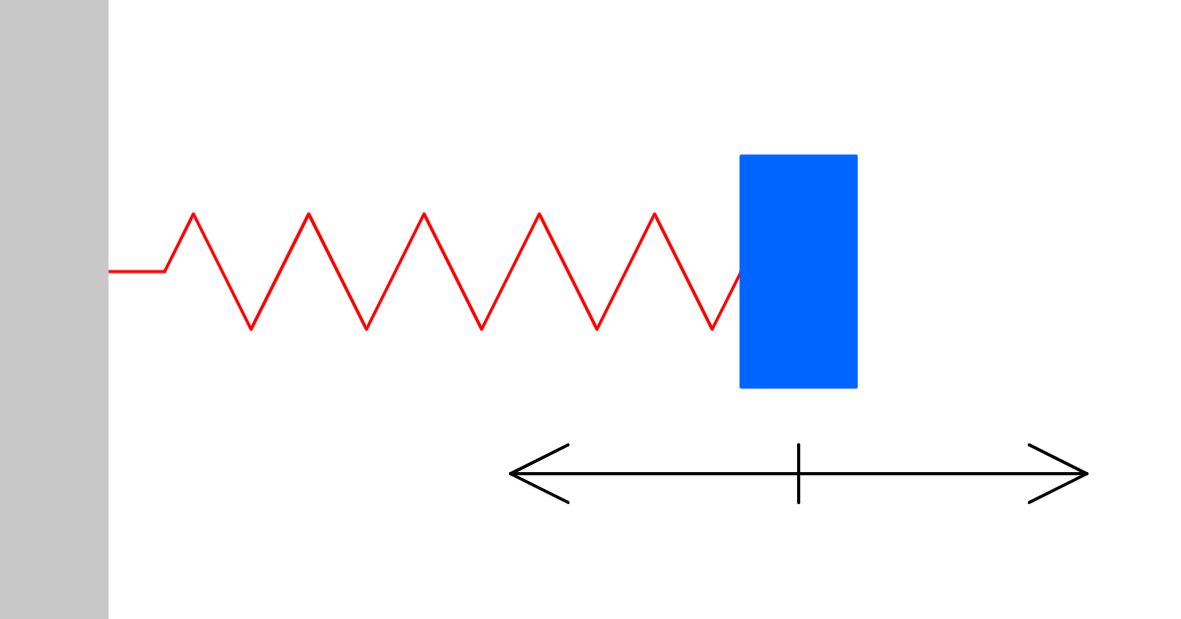
\includegraphics[width=11cm]{Spring Mass Damper.png}
\caption{Spring-Mass-Damper.}
\label{fig:spring-mass}
\end{figure}

Letting $u = -Kx$, this becomes
$$\dx = (A - BK)x$$ 
where $K \in \mathbb{R}^{1 \times 2}$, so we can write $K = \begin{pmatrix} k_1 & k_2 \end{pmatrix}$. Evaluating $A - BK$, we get
$$A - BK = \begin{pmatrix} 0 & 1 \\ -2 & 3 \end{pmatrix} - \begin{pmatrix} 0 \\ 1 \end{pmatrix}\begin{pmatrix} k_1 & k_2 \end{pmatrix} = \begin{pmatrix} 0 & 1 \\ -2 & 3 \end{pmatrix} - \begin{pmatrix} 0 & 0 \\ k_1 & k_2 \end{pmatrix} = \begin{pmatrix} 0 & 1 \\ -2 - k_1 & 3 - k_2 \end{pmatrix}.$$
Evaluating the eigenvalues, we see that they satisfy the characteristic equation $\det(\lambda I - (A - BK)) = 0$, or
$$\lambda^2 + (k_2 - 3)\lambda + (k_1 + 2) = 0.$$
Now, we arbitrarily choose the (negative) eigenvalues, say $-2, -5$. They would satisfy $(\lambda + 2)(\lambda + 5) = \lambda^2 + 7\lambda + 10 = 0$. We want the eigenvalues to match, so the coefficients must match too, and we have:
\begin{align*}
k_1 + 2 = 10 \implies k_1 = 8 \\
k_2 - 3 = 7 \implies k_2 = 10
\end{align*}
so $K = \begin{pmatrix} 8 & 10 \end{pmatrix}$, and $u = \begin{pmatrix} 8 & 10 \end{pmatrix}x$ makes the system stable.

\subsection{Nonlinear Dynamics and Control}

Similar to how we linearize systems without a control, we can approximate nonlinear systems with a control as a linear system. \\

Consider a general nonlinear dynamical system with control inputs:
$$\dx = f(x, u).$$
A fixed point $(x^*, u^*)$ satisfies $f(x^*, u^*) = 0$. \\

Define small perturbations around the fixed point:
$$\Delta x = x - x^*, \quad \Delta u = u - u^*.$$
Then, we can approximate $\Delta \dx = f(x, u)$ using a Taylor expansion around $(x^*, u^*)$:
$$f(x, u) \approx f(x^*, u^*) + A\Delta x + B\Delta u$$
where
$$A = \left. \frac{\partial f}{\partial x}\right|_{(x^*, u^*)}, \quad B = \left. \frac{\partial f}{\partial u}\right|_{(x^*, u^*)}$$
are the Jacobian matrices of $f$ with respect to the state vector $x$ and control vector $u$. Since $f(x^*, u^*) = 0$, this simplifies to
$$\Delta \dx \approx A\Delta x + B\Delta u$$
which we can then use linear methods to analyze stability on. \\

Again, we can assume that if the eigenvalues of the system matrix are negative then the fixed point of the nonlinear system is stable. \\

Let's look at an example to illustrate the process. Consider the nonlinear system with control described by:
$$\dx_1 = x_1^2 + x_2 + u$$ $$\dx_2 = x_1 + \sin(x_2).$$
Suppose the fixed point is $(x_1^*, x_2^*, u^*) = \left(0, 0, 0\right)$. We can write $f$ as
$$f(x, u) = \begin{pmatrix} x_1^2 + x_2 + u \\ x_1 + \sin(x_2) \end{pmatrix}.$$
The Jacobian matrices are
$$A = \left. \frac{\partial f}{\partial x} \right|_{(0, 0, 0)} = \begin{pmatrix} \frac{\partial (x_1^2 + x_2 + u)}{\partial x_1} & \frac{\partial (x_1^2 + x_2 + u)}{\partial x_2} \\ \frac{\partial (x_1 + \sin(x_2))}{\partial x_1} & \frac{\partial (x_1 + \sin(x_2))}{\partial x_2} \end{pmatrix} = \begin{pmatrix} 0 & 1 \\ 1 & \cos(0) \end{pmatrix} = \begin{pmatrix} 0 & 1 \\ 1 & 1 \end{pmatrix},$$
$$B = \left. \frac{\partial f}{\partial u} \right|_{(0, 0, 0)} = \begin{pmatrix} \frac{\partial (x_1^2 + x_2 + u)}{\partial u} \\ \frac{\partial (x_1 + \sin(x_2))}{\partial u} \end{pmatrix} = \begin{pmatrix} 1 \\ 0 \end{pmatrix}.$$ So the final linearized system is $$\Delta \dx = \begin{pmatrix} 0 & 1 \\ 1 & 1 \end{pmatrix}\Delta x + \begin{pmatrix} 1 \\ 0 \end{pmatrix}\Delta u.$$
The stability of this system can now be analyzed using the standard techniques for linear systems with control that we just covered.

\section{Cart-Pole Problem}

One classic problem in control theory is the cart-pole problem. It is a system where a cart can travel in the $x$ direction and it needs to balance a pole attached to it with a pin joint. \\

Figure \ref{fig:cart-pole} shows a simplified model of the Cart-Pole problem. The variables are:
\begin{itemize}
\item $x$: Position of the cart
\item $\theta$: Angle of the pole (upright position is $\theta = 0$)
\item $u: \text{Control force applied to the cart}$
\item $M: \text{Mass of the cart}$
\item $m: \text{Mass of the pole}$
\item $l: \text{Length of the pole}$
\item $g: \text{Acceleration due to gravity}$
\end{itemize}

\begin{figure}
\centering
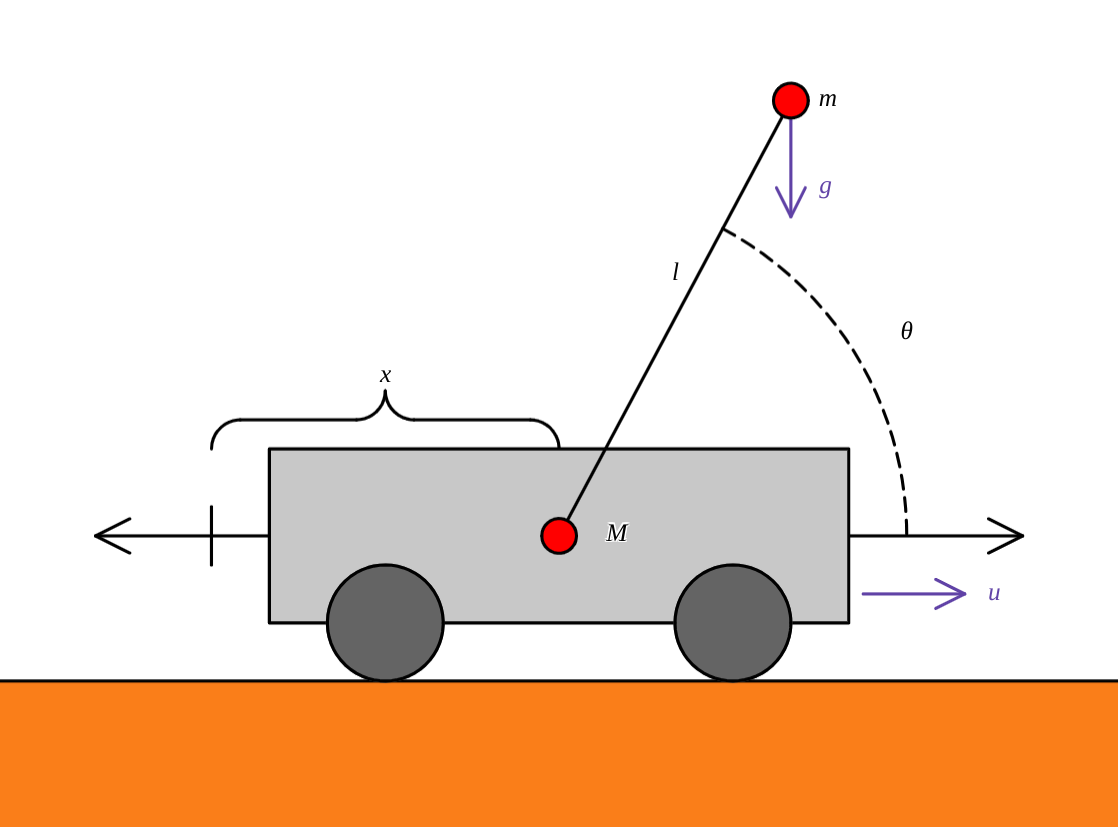
\includegraphics[width=11cm]{Cart-Pole Problem.png}
\caption{The cart-pole problem.}
\label{fig:cart-pole}
\end{figure}

Using mechanics (namely Newton's second law of motion and Lagrangian mechanics), we can derive the equations: \cite{Cart-Pole}
\begin{align*}
& (M + m)\ddx + ml\ddth\cos(\theta) - ml\dth^2\sin(\theta) = u \\
& l\ddth + g\sin(\theta) = \ddx\cos(\theta).
\end{align*}
The first equation models the horizontal force of the cart and the second one models the rotational force of the pole. The fixed point is where the pole is vertical, so $\theta = 0$. Now, we linearize the equations of motion around the fixed point. \\

The state vector is $\bx = \begin{pmatrix} x_1 \\ x_2 \\ x_3 \\ x_4 \end{pmatrix} = \begin{pmatrix} x \\ \dx \\ \theta \\ \dth \end{pmatrix}$. We can make the approximations
\begin{align*}
\sin(\theta) \approx \theta \\
\cos(\theta) \approx 1
\end{align*}
for $\theta$ sufficiently close to $0$. Substituting those into the original equations, we have
\begin{align*}
(M + m)\ddx + ml\ddth - ml\dot{\theta}^2\theta &\approx u \\
l\ddth + g\theta &\approx \ddx.
\end{align*}
Since we are linearizing the system around $\bx = 0$, we can assume $\theta$ and $\dth$ are close to $0$ and neglect higher order terms like $\dth^2\theta$, which gives us
\begin{align}
\label{eq:1}
(M + m)\ddx + ml\ddth &\approx u \\
\label{eq:2}
l\ddth + g\theta &\approx \ddx.
\end{align}
We want to write this in the form
$$\dbx = \begin{pmatrix} \dx \\ \ddx \\ \dth \\ \ddth \end{pmatrix} \approx \begin{pmatrix} \dx_1 \\ \dx_2 \\ \dx_3 \\ \dx_4 \end{pmatrix} = f(\bx, u).$$
We can start by finding an expression for $\dx_1$ in terms of the other components. We see that $\dx_1 = \dx = x_2$. \\

Now, we can find an expression for the second component. Using (\ref{eq:2}), we have
$$\dx_2 = \ddx = l\ddth + g\theta.$$
Moving onto the third component, we have that $\dx_3 = \dot{\theta} = x_4$. \\
Finally, isolating $\ddth$ in (\ref{eq:2}) gives us
$$\dx_4 = \ddth = \frac{\ddx - g\theta}{l}.$$
We have that $\ddx = l\ddth + g\theta$ and isolating $\ddx$ in (\ref{eq:1}) gives us $\ddx = \frac{u - ml\ddth}{M + m}$. Solving this for $\ddth$, we have
$$\ddth = \frac{u - Mg\theta - mg\theta}{l(M + 2m)}$$
and substituting into $\ddx = l\ddth + g\theta$ and simplifying gives us
$$\ddx = \frac{u + mg\theta}{M + 2m}.$$
So we have that
$$\dx_2 = \ddx = \frac{u + mg\theta}{M + 2m} = \frac{u + mgx_3}{M + 2m}$$
and
$$\dx_4 = \ddth = \frac{u - Mg\theta - mg\theta}{l(M + 2m)} = \frac{u - Mgx_3 - mgx_3}{l(M + 2m)}.$$
This gives us $$f(\bx, u) = \begin{pmatrix} x_2 \\ \dfrac{u + mgx_3}{M + 2m} \\ x_4 \\ \dfrac{u - Mgx_3 - mgx_3}{l(M + 2m)} \end{pmatrix}.$$
This function gives us an expression for the rates of change of each component in the state vector. \\

Now, we need to find the Jacobian matrices of $f$ with respect to $\bx$ and $u$. We find that
$$A = \frac{\partial f}{\partial \bx} = 
\begin{pmatrix}
0 & 1 & 0 & 0 \\
0 & 0 & \frac{mg}{M + 2m} & 0 \\
0 & 0 & 0 & 1 \\
0 & 0 & -\frac{Mg + mg}{l(M + 2m)} & 0
\end{pmatrix}$$
and $$B = \frac{\partial f}{\partial u} =
\begin{pmatrix}
0 \\
\frac{1}{M + 2m} \\
0 \\
\frac{1}{l(M + 2m)}
\end{pmatrix}.$$
This gives us
$$\dbx \approx A\bx + Bu$$
where $A$ and $B$ are as derived above. \\

Now, let
$$u = -Kx.$$
This gives us
$$\dbx \approx (A - BK)\bx.$$
Since $K \in \mathbb{R}^{1 \times 4}$, letting
$$K =
\begin{pmatrix}
k_1 & k_2 & k_3 & k_4
\end{pmatrix}$$
and solving the characteristic equation $$\det(A - BK) = 0$$ will reveal which matrices $K$ keep the system stable. \\

Unfortunately, evaluating the determinant of a $4\times 4$ matrix is extremely tedious to do by hand, and solving the resulting polynomial would most likely require numerical methods. When working with nonlinear systems, complete solutions often require computational approaches. Some examples are the \textbf{QR algorithm} \cite{Van23} and the \textbf{power method} \cite{Numerical-Eigenvalue}. \\

Taking a step back, we see that what we have done allows us to make the cart move in a way that depends only on the position of the cart, the angle of the pole, and the rates of change of both, while guaranteeing that the pole will be kept upright. This example highlights the importance of stability analysis in robotics and control theory.

\section{Future Work - Lyapunov's Direct Method}

In this paper, we mainly dealt with nonlinear systems by linearizing them and then using linear methods to analyze those systems. However, there is another, more powerful method to analyze stability that doesn't require linearization. This is called Lyapunov's direct method. It involves constructing a function that can provide insights, not only into the stability of a fixed point, but also the properties of the nonlinear system. Here are some sources if you want to explore further: \cite{Lya-Direct, Lya-Indirect}.

\bibliographystyle{alpha}
\bibliography{biblio}

\end{document}